\subsection{Sleep modes}

\subsubsection{Experimental setup}
A common use case of a battery powered device is a temperature sensor.
Therefore, we used the following experimental setup:
\textit{The device should measure the temperature with an interval of $T_{measure} = 15min$.
MQTT should be used to publish the measured data to other devices.}

Fig. \ref{fig:experiment_modem_light_sleep} represents the test programm for the modem and light sleep.
The step \textit{setRandomMacAddress} makes sure that the ESP8266 always gets a new IP address.

\begin{figure}[h]
    \centering
    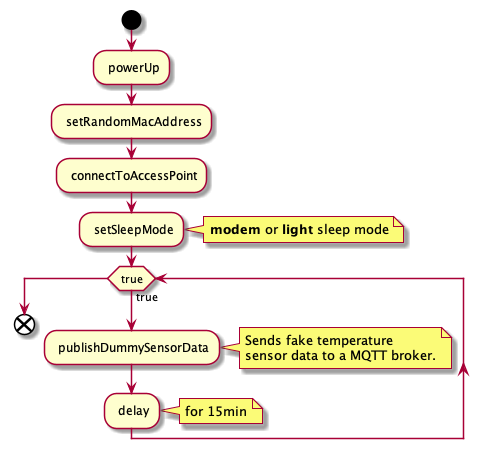
\includegraphics[width = 0.7 \linewidth]{fig/sequence_modem_light_sleep.png}
    \caption{Experimental setup for modem and light sleep.}
    \label{fig:experiment_modem_light_sleep}
\end{figure}

Fig. \ref{fig:experiment_deep_sleep} describes the experimental setup that was used to perform tests on the deep sleep mode.
After the \textit{enterDeepSleep} step, the ESP8266 sleeps for $15min$ and starts the sequence again.
The difference between deep sleep and modem / light sleep mode is, that the controller restarts the programm everytime it wakes up from the deep sleep mode.
\begin{figure}[h]
    \centering
    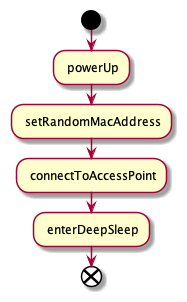
\includegraphics[width = 0.7 \linewidth]{fig/sequence_deep_sleep.png}
    \caption{Experimental setup for deep sleep.}
    \label{fig:experiment_deep_sleep}
\end{figure}

\subsubsection{Modem sleep}
As mentioned in TODO, the ESP8266 automatically disables the modem when there is no data transmission required.
During transmission the module takes around $80mA$. During modem sleep, $20mA$ are needed.
The modem wakes up every $100ms$ to keep the connection to the access point established.
Fig. \ref{fig:beacon_interval} shows the beacon interval of $100ms$. 
The same behavior was observed in \cite{montori_is_2017}.

\begin{figure}[h]
    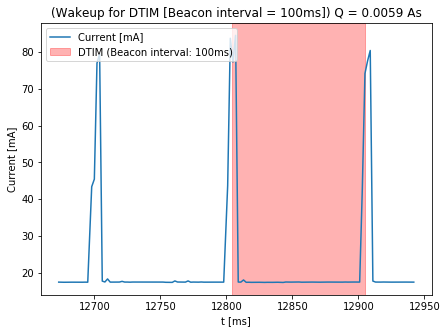
\includegraphics[width = \linewidth]{fig/beacon_interval.png}
    \caption{The power consumption increases to $\approx 80mA$, everytime a beacon arrives.}
    \label{fig:beacon_interval}
\end{figure}

\subsubsection{Light sleep}
As described in TODO, the light sleep mode disables the CPU when no task has to be processed.
When a task has to be processed, the ESP8266 switches back into modem sleep.
Fig. \ref{tab_sleep_modes} shows the change from light sleep (green) to modem sleep (red).
It is clear to see that the ESP8266 still needs a lot of power when a beacon arrives (every $100ms$).

\begin{figure}[h]
    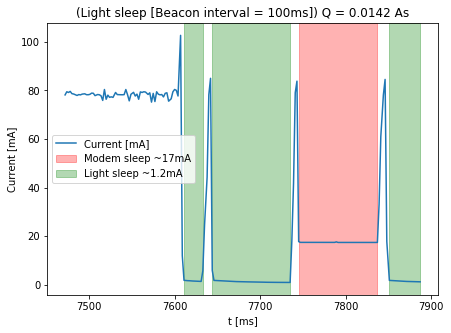
\includegraphics[width = \linewidth]{fig/light_sleep.png}
    \caption{During the light sleep mode, the power consumption of the ESP8266 is drops to 1.2mA.}
    \label{fig:light_sleep}
\end{figure}

\subsubsection{Deep sleep}
The deep sleep mode is the most efficient sleep mode, as described in TODO. 
We achieved a power consumption of only $20 \mu A$. 
However, the ESP8266 takes a long time to reconnect to the WiFi network after the sleep phase.
Fig. \ref{fig:deep_sleep} shows the power consumtion during sleep and wake phase.
\begin{figure}[h]
    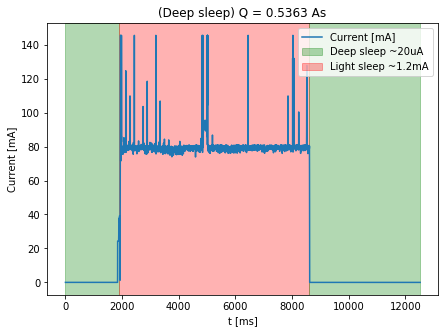
\includegraphics[width = \linewidth]{fig/deep_sleep.png}
    \caption{During deep sleep mode (green), the power consumption drops to $16 \mu A$}
    \label{fig:deep_sleep}
\end{figure}